\begin{frame}{Af hverju þetta námsefni?}
	\begin{itemize}
		\item Það sem eftir er af námskeiðinu snýst um þekkt reiknirit \eng{algorithms} og gagnagrindur \eng{data structures}
		      \begin{itemize}
			      \item Fræðilegt!
		      \end{itemize}
		\item Fátt sem kemur jafn víða við, þó e.t.v. munið þið ekki koma til með að útfæra grundvallarreiknirit sjálf
		      \begin{itemize}
			      \item Gagnlegt að vita hvernig innbyggð reiknirit virka
			      \item Innsýn mun nýtast í öðrum samhengjum
		      \end{itemize}
		\item Almennara en aðrar leiðir til að læra forritun
	\end{itemize}
\end{frame}

\begin{frame}{Vandamál!}
	\begin{itemize}
		\item Skil geta verið\ldots
		      \begin{itemize}
			      \item \ldots of erfið í útfærslu
			      \item \ldots of erfið í notkun
			      \item \ldots of þröng (of fáar aðferðir)
			      \item \ldots of víð (of margar aðferðir)
			      \item \ldots of almenn
			      \item \ldots of sérhæfð
			      \item \ldots of háð útfærslunni
		      \end{itemize}
		\item En samt nauðsynleg!
	\end{itemize}
\end{frame}

\section{Fleiri gagnagerðir}

\subsection{Strengir}

\begin{frame}{\texttt{string}}
    \begin{itemize}
        \item Við þurfum oft að vinna með texta, til þess er hægt að nota gagnagerðina \texttt{char}
        \begin{itemize}
            \item Til að fá strengi með \texttt{char} þarf að nota fylki af táknum
            \item Fylki af táknum eru ekki jafn meðfærileg og við búumst við af strengjum úr öðrum forritunarmálum 
        \end{itemize}
        \item Líkt og \texttt{std::vector} gerir almenna fylkjavinnslu þægilegri gerir \texttt{std::string} sérhæfða strengjavinnslu þægilegri
    \end{itemize}
\end{frame}

\begin{frame}{Kostir \texttt{string}}
\begin{itemize}
    \item Líkt og \texttt{vector} sér \texttt{string} um sína eigin minnisstjórnun
    \begin{itemize}
    \item Í C++11, gert mjög vel
    \end{itemize}
    \item Innbyggðir virkjar
    \item Innbyggð föll
\end{itemize}
\end{frame}

\begin{frame}{Hvað er hægt að gera við \texttt{string}?}
\cppfile[firstline=7, lastline=11, label=stringtricks.cpp]{Code/w3/stringtricks.cpp}
\cppfile[firstline=15, lastline=20, label=stringtricks.cpp]{Code/w3/stringtricks.cpp}
\end{frame}

\begin{frame}{Hvað er hægt að gera við \texttt{string}?}
\cppfile[firstline=24, lastline=27, label=stringtricks.cpp]{Code/w3/stringtricks.cpp}
\cppfile[firstline=31, lastline=34, label=stringtricks.cpp]{Code/w3/stringtricks.cpp}
\end{frame}


\subsection{Mengi}

\begin{frame}{Mengi}
\texttt{std::set} skilgreinir mengi staka, án endurtekninga. \texttt{std::multiset} skilgreinir safn staka, með endurtekningum.

\begin{center}
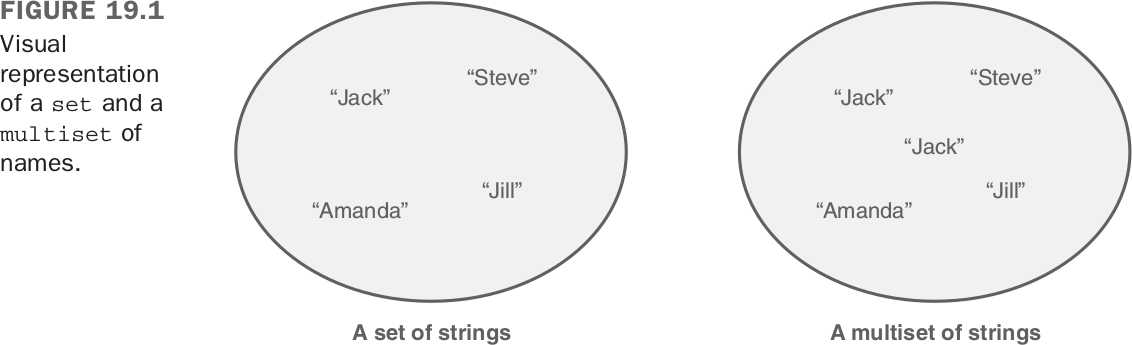
\includegraphics[width=\textwidth]{set-multiset}
\end{center}


Ólíkt þeim mengjum sem við þekkjum úr stærðfræði eru þessi mengi röðuð!
\end{frame}

\begin{frame}{Röðuð og óröðuð mengi}
\begin{itemize}
\item \texttt{set} og \texttt{multiset} eru skilgreind í \texttt{<set>}
\begin{itemize}
\item Til að hægt sé að setja klasa sem við höfum skrifað í þessi mengi þurfa þeir að vera samanberanlegir
\item Fjölbinding fyrir < virkjann!
\end{itemize}
\item Nýtt í C++11: \texttt{unordered\_set} og \texttt{unordered\_multiset} eru skilgreind í \texttt{<unordered\_set>}
\begin{itemize}
\item Þurfum að útfæra \href{http://en.cppreference.com/w/cpp/utility/hash}{hakkafall} fyrir klasana okkar til að hægt sé að geyma þá í óröðuðum mengjum
\end{itemize}
\item Aðgerðir á mengin hafa mismundandi tímaflækjur
\item Munum kynnast þessum betur síðar
\end{itemize}
\end{frame}

\subsection{Varpanir}

\begin{frame}{Varpanir}
\begin{columns}
\column{0.4\textwidth}
\begin{itemize}
\item \texttt{std::map} og \texttt{std::multimap} tengja saman lykla (e. \emph{keys}) og gildi (e. \emph{values})
\item Skoðum \texttt{multimapexample.cpp}
\end{itemize}
\column{0.6\textwidth}
\begin{center}
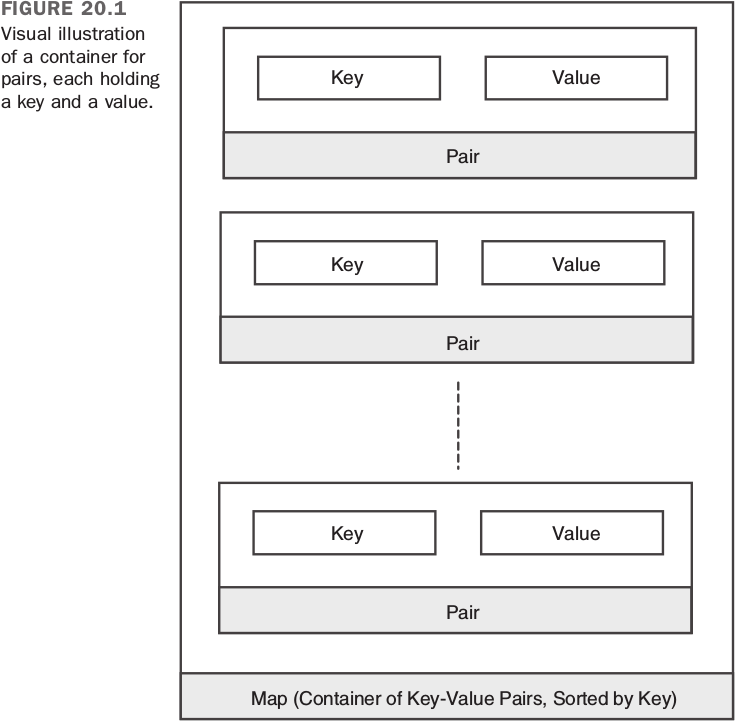
\includegraphics[width=\linewidth]{map}
\end{center}
\end{columns}
\end{frame}